% Start backup slides
\section*{Backup Slides}
\backupbegin

\begin{comment}

\begin{frame}{High-Performance FPGA-Based CNN Accelerator With Block-Floating-Point Arithmetic}
\centering
\begin{figure}
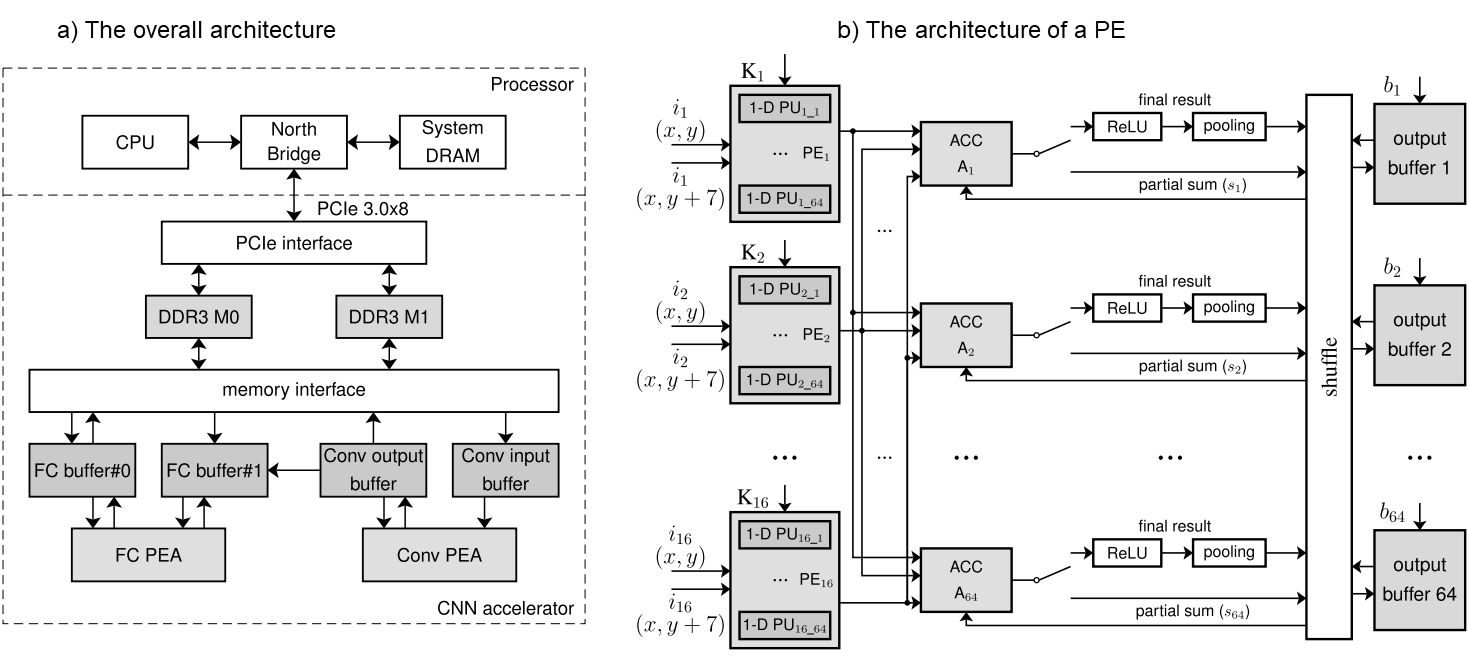
\includegraphics[width=\textwidth]{../figures/3_g.png}
\caption{(a) System architecture. (b) Processing element array.}
\end{figure}
\end{frame}

\begin{frame}{A 200MHZ 202.4GFLOPS@10.8W VGG16 Accelerator in Xilinx VX690T}
\centering
\begin{figure}
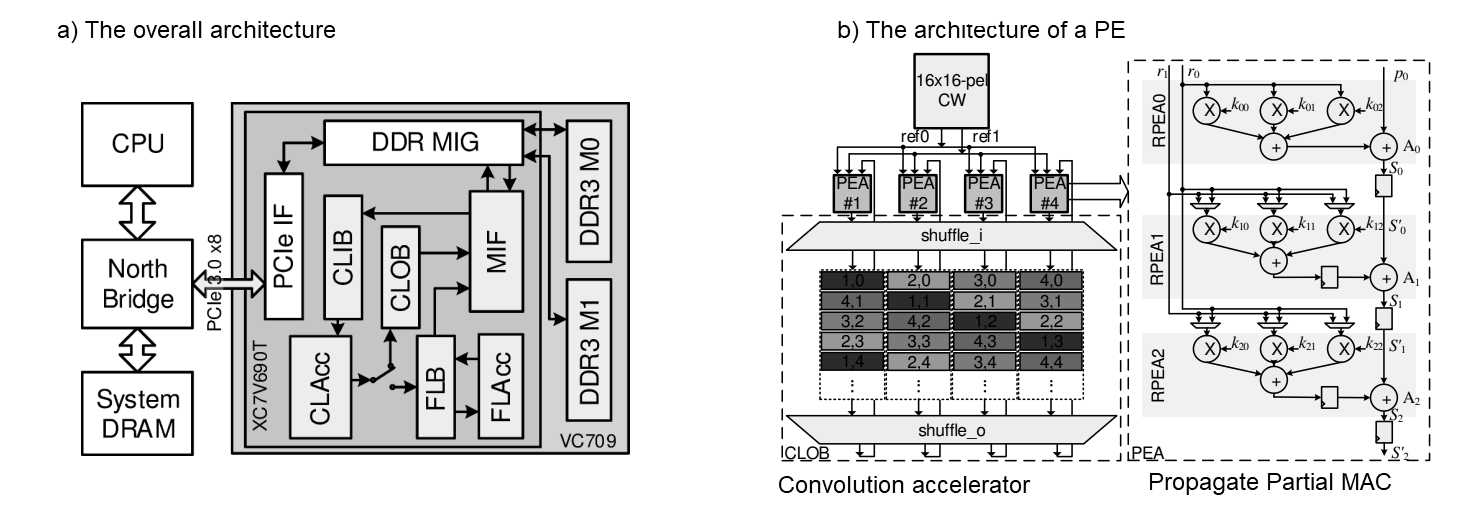
\includegraphics[width=\textwidth]{../figures/1_g.png}
\caption{(a) System architecture. (b) Convolution accelerator.}
\end{figure}
\end{frame}

\begin{frame}{Low-precision Floating-point Arithmetic for High-performance FPGA-based CNN Acceleration}
\centering
\begin{figure}
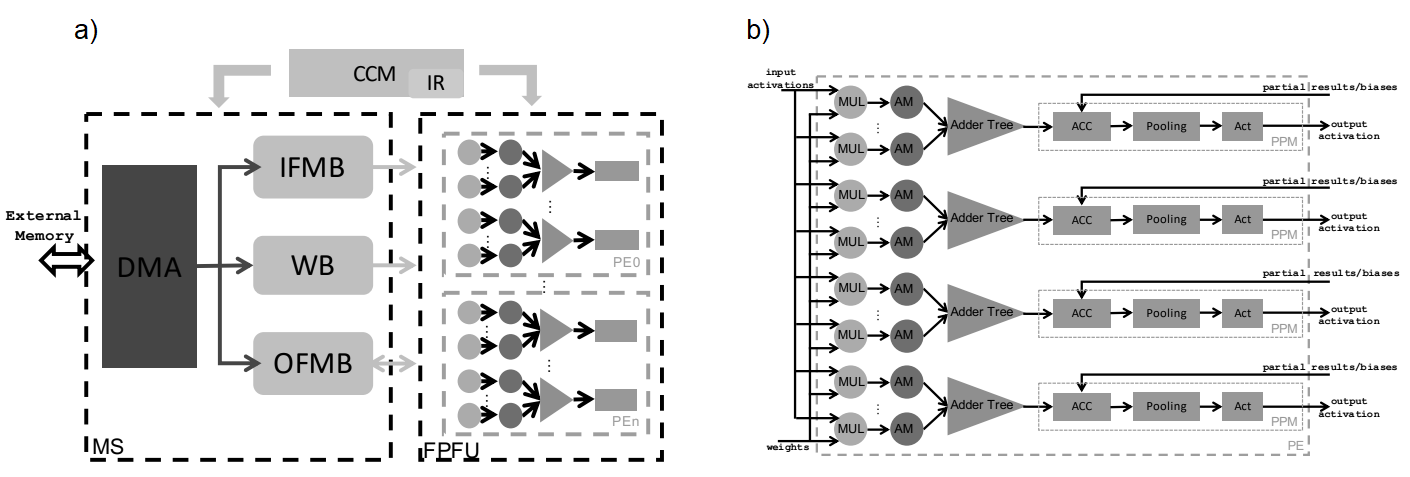
\includegraphics[width=\textwidth]{../figures/2_g.png}
\caption{(a) System architecture. (b) Processing element.}
\end{figure}
\end{frame}

\begin{frame}{CNN Hardware Acceleration on a Low-Power and Low-Cost APSoC}
\centering
\begin{figure}
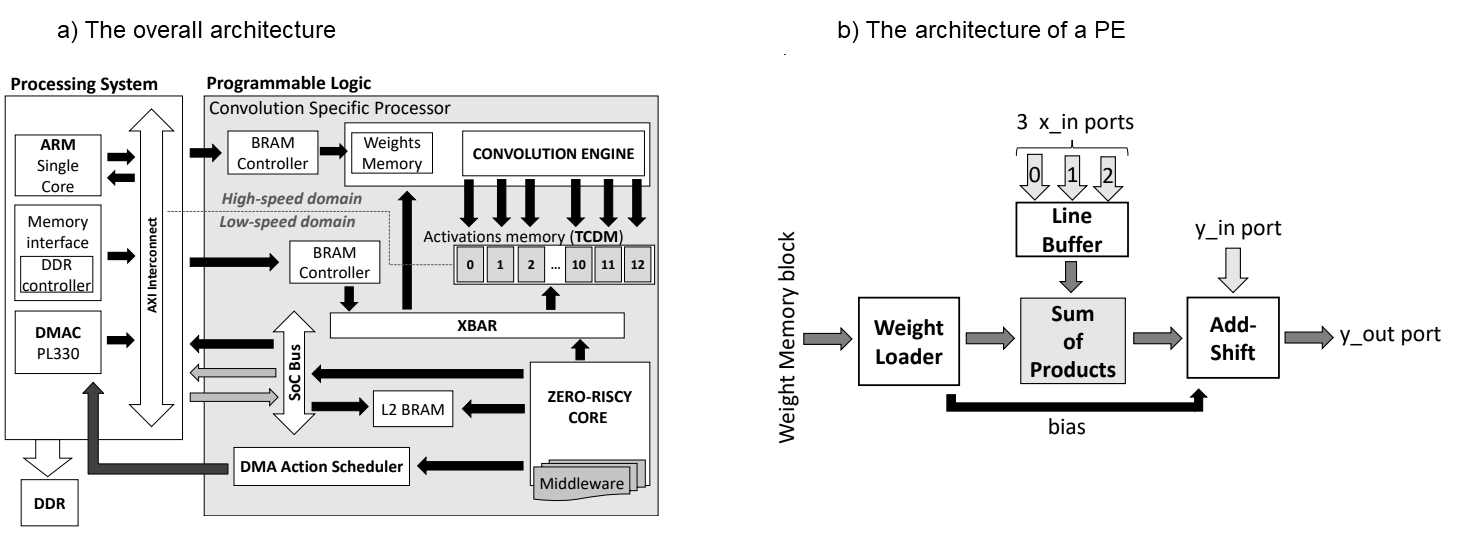
\includegraphics[width=\textwidth]{../figures/4_g.png}
\caption{(a) System architecture. (b) Convolution engine.}
\end{figure}
\end{frame}

\end{comment}


\begin{frame}{Limitations of State-of-the-Art}
	\begin{itemize}
		\item<1-> \textbf{Spike-by-Spike Neural Networks:}
		\begin{itemize}
			\item<2-> \alert{Quantization Challenges:} Struggles with reduced number representations (8-bit and 4-bit)
			\item<3-> \alert{Deployment Frameworks:} Lack of deployment strategies for IoT and TinyML applications
			\item<4-> \alert{Design Methodologies:} Lack of effective low-power accelerator design methodologies
		\end{itemize}
		\item<5-> \textbf{Low-Power CNN Accelerators:}
		\begin{itemize}
			\item<6-> \alert{Floating-Point Design:} Literature gap in floating-point methodologies for IoT and TinyML applications
			\item<7-> \alert{Reproducibility:} Deficiency in reproducible research, limiting validation and adoption
		\end{itemize}
		\item<8-> \textbf{Low-Power Accelerators with Aggressive Quantization:}
		\begin{itemize}
			\item<9-> \alert{Computational Efficiency vs. Accuracy:} Enhances efficiency but often at the expense of significant accuracy degradation in complex tasks
			\item<10-> \alert{Mission-Critical Applications:} Often unsuitable for applications requiring high reliability, safety, and quality-of-result
			\item<11-> \alert{Compatibility and Portability:} Faces challenges in compatibility and portability across different computing platforms and ML frameworks
		\end{itemize}
	\end{itemize}
\end{frame}

\begin{frame}{Spike-by-Spike Neural Network}

			\begin{figure}
				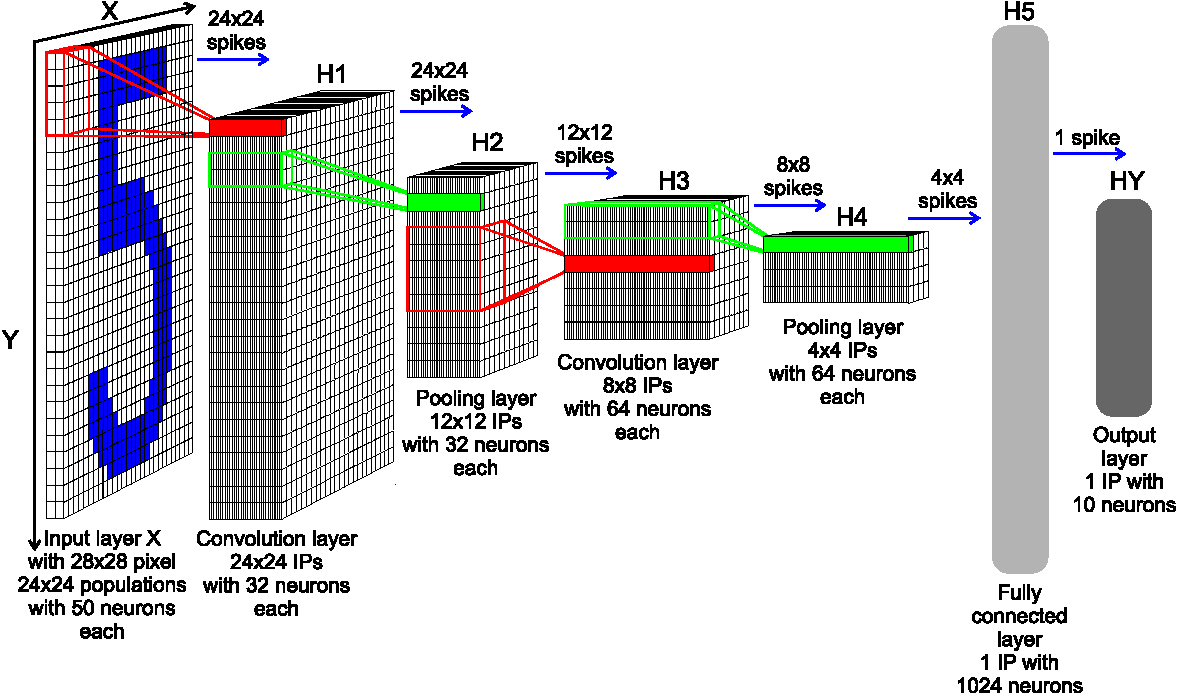
\includegraphics[width=0.9\textwidth]{../chapters/sbs_accelerator/figures/sbs_network.pdf} % Adjust the filename
				\caption{Spike-by-Spike (SbS) neural network architecture for handwritten digit classification task}
			\end{figure}

\end{frame}

\begin{frame}{SbS Processing Unit}
	\begin{columns}[c] % The [T] option aligns the tops of the columns
		
		% Left column for the first image
		\begin{column}<1->{0.5\textwidth}
			\begin{figure}
				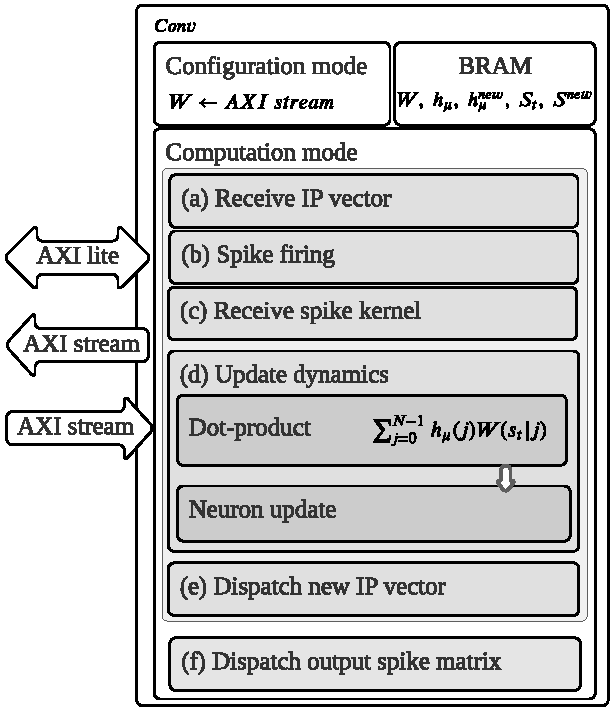
\includegraphics[width=0.7\textwidth]{../chapters/sbs_accelerator/figures/sbs_conv.pdf} % Adjust the filename
				\caption{Convolution processing unit}
			\end{figure}
		\end{column}
		
		% Right column for the second image
		\begin{column}<2->{0.5\textwidth}
			\begin{figure}
				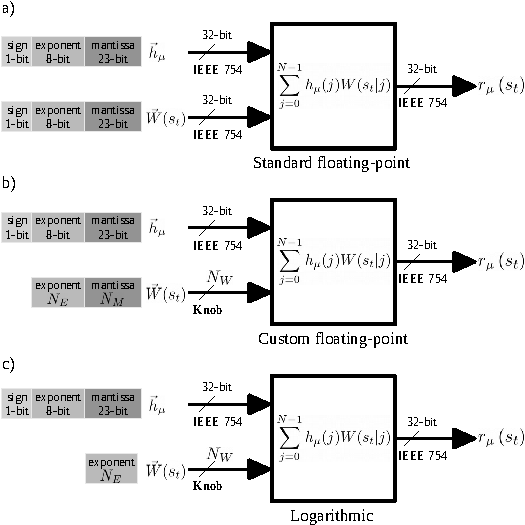
\includegraphics[width=0.9\textwidth]{../chapters/sbs_accelerator/figures/dot-product_unit.pdf} % Adjust the filename
				\caption{Dot-product hardware module}
			\end{figure}
		\end{column}
		
	\end{columns}
\end{frame}


\begin{frame}{SbS HW/SW Co-Design and Deployment Framework}
	
	\begin{figure}
		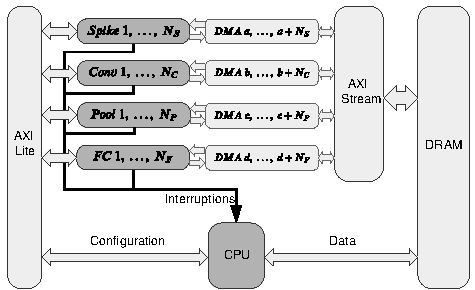
\includegraphics[width=0.75\textwidth]{./slides/figures/sbs_hw.pdf} % Adjust the filename
		\caption{System-level hardware architecture with scalable number of heterogeneous processing units}
	\end{figure}
	
\end{frame}

\begin{frame}{Hybrid Dot-Product Approximation}
	\begin{columns}[t] % The [T] option aligns the tops of the columns
		% Left column for equations
		\begin{column}{0.5\textwidth}
			
			\begin{equation}
			r_{\mu}\left(s_t\right)=\sum_{j=0}^{N-1}h_{\mu}(j)W(s_t|j)
			\end{equation}
			\vspace{4mm} 
			\begin{equation}
			E_{\min}=\log _2(\min_{\forall i}(W(i)))
			\end{equation}
			\vspace{4mm} 
			\begin{equation}
			N_E=\lceil\log_2(|E_{\min}|)\rceil
			\end{equation}
			\vspace{4mm} 
			\begin{equation}
			N_W=N_E + N_M
			\end{equation}
		\end{column}
		
		% Right column for the image
		\begin{column}{0.5\textwidth}
			\begin{figure}
				\centering
				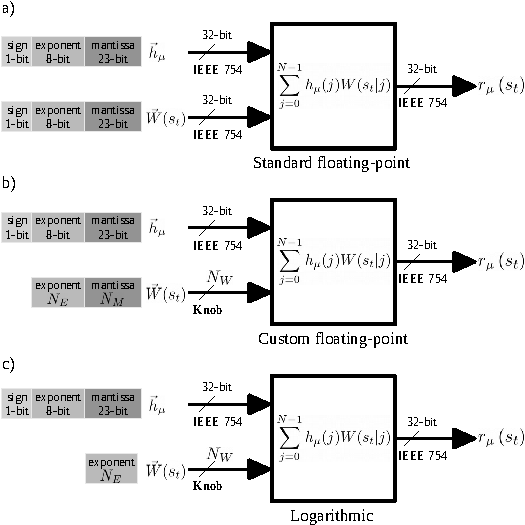
\includegraphics[width=0.9\textwidth]{../chapters/sbs_accelerator/figures/dot-product_unit.pdf} % Adjust the filename
				\caption{Dot-product hardware module}
			\end{figure}
		\end{column}
	\end{columns}
\end{frame}

\begin{frame}{Dot-Product with Standard Floating-Point (IEEE 754)}
	\begin{figure}
		\centering
		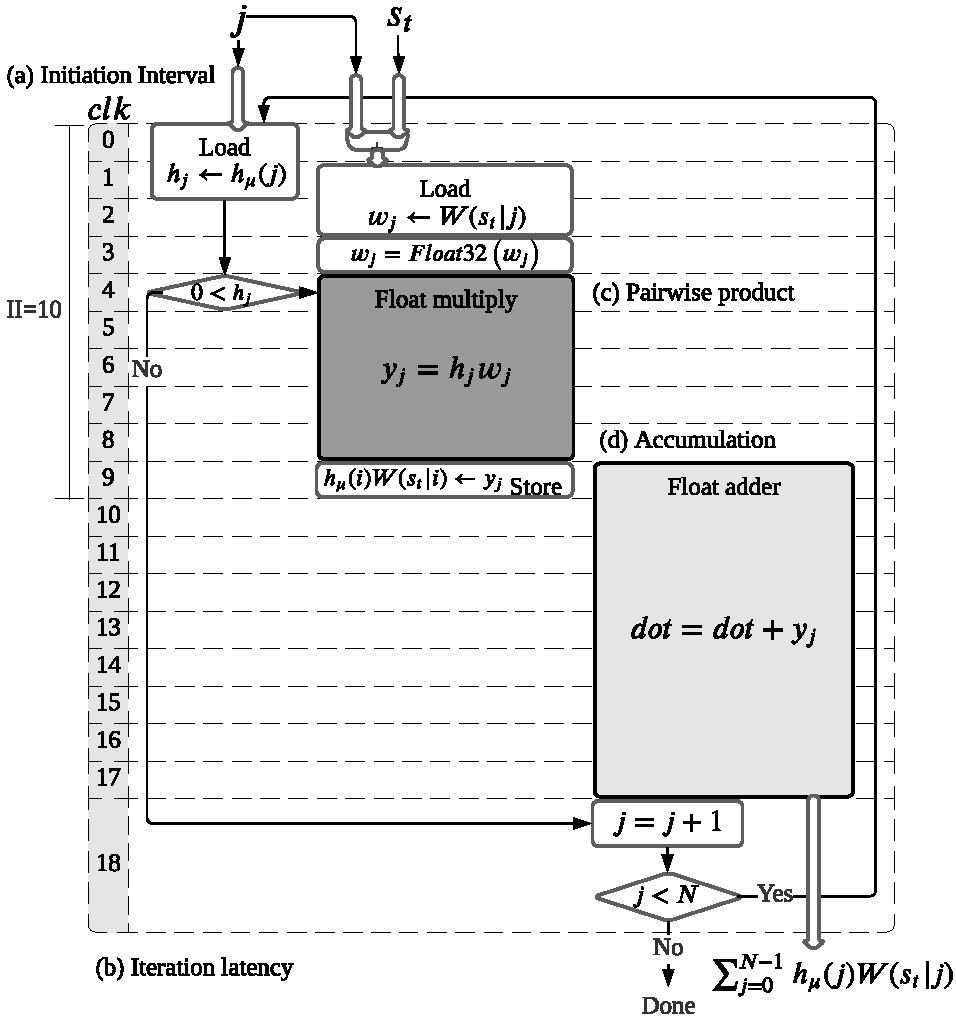
\includegraphics[width=0.4\columnwidth]{../chapters/sbs_accelerator/figures/dot_product_float.pdf}
		\caption{Dot-product hardware module with standard floating-point computation}
	\end{figure}
	
	\vfill % Add vertical space to push the equation to the bottom
	
	% Equation at the bottom
	\[
	L_{f32}=10N+9
	\]
\end{frame}

\begin{frame}{Dot-Product with Hybrid Custom Floating-Point Approximation}
	\begin{figure}
		\centering
		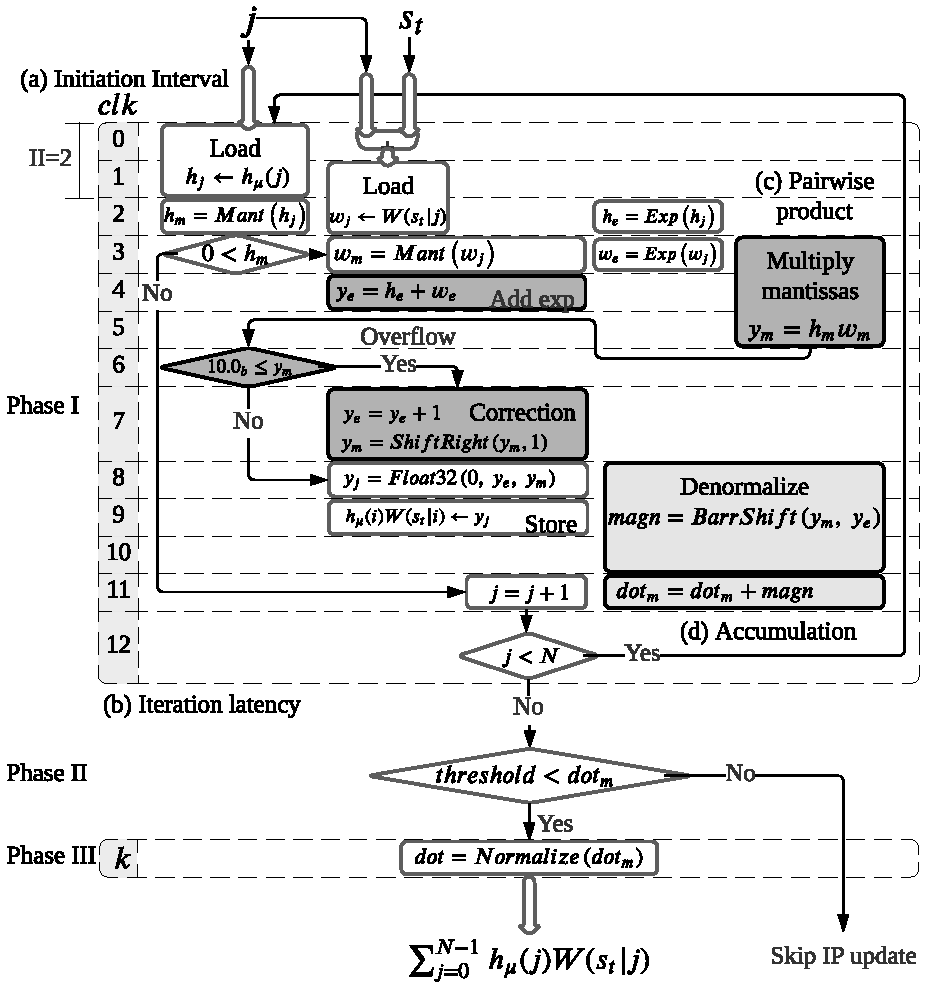
\includegraphics[width=0.4\columnwidth]{../chapters/sbs_accelerator/figures/dot_product.pdf}
		\caption{Dot-product hardware module with hybrid custom floating-point approximation}
	\end{figure}
	
	\vfill % Add vertical space to push the equation to the bottom
	
	% Equation at the bottom
	\[
	L_{custom}=2N+11
	\]
\end{frame}

\begin{frame}{Dot-product with Hybrid Logarithmic Approximation}
	\begin{figure}
		\centering
		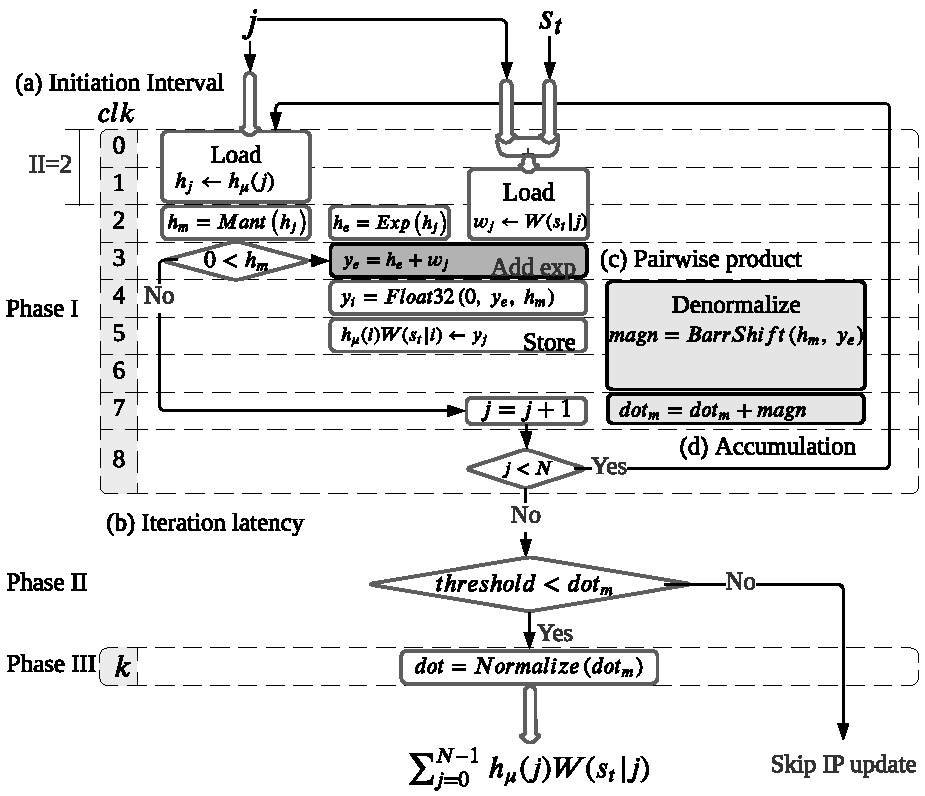
\includegraphics[width=0.4\columnwidth]{../chapters/sbs_accelerator/figures/dot_product_log.pdf}
		\caption{Dot-product hardware module with hybrid logarithmic approximation}
	\end{figure}
	
	\vfill % Add vertical space to push the equation to the bottom
	
	% Equation at the bottom
	\[
	L_{custom}=2N+7
	\]
\end{frame}

\begin{frame}{Deployment with Standard Floating-Point}
	\begin{columns}
		% Left Column
		\begin{column}{0.5\textwidth}
			% Top left image
			\begin{minipage}[c][.45\textheight][c]{\linewidth}
				\centering
				\begin{figure}
					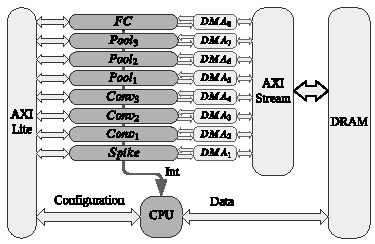
\includegraphics[width=0.75\linewidth]{./slides/figures/sbs_hw_experimental.pdf} % Adjust path and size as needed
					\caption{System overview of the top-level architecture with 8 processing units}
				\end{figure}
				\pause
			\end{minipage}
			
			% Bottom left image
			\begin{minipage}[c][.45\textheight][c]{\linewidth}
				\centering
				\begin{figure}
					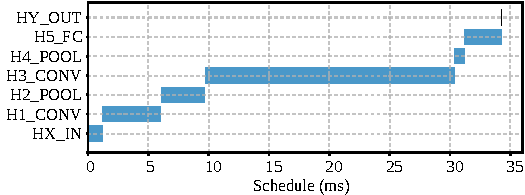
\includegraphics[width=0.75\linewidth]{../chapters/sbs_accelerator/figures/latency_sw.pdf} % Adjust path and size as needed
					\caption{Computation on embedded CPU}
				\end{figure}
				\pause
			\end{minipage}
		\end{column}
		
		% Right Column
		\begin{column}{0.5\textwidth}
			% Top right image
			\begin{minipage}[c][.45\textheight][c]{\linewidth}
				\centering
				\begin{figure}
					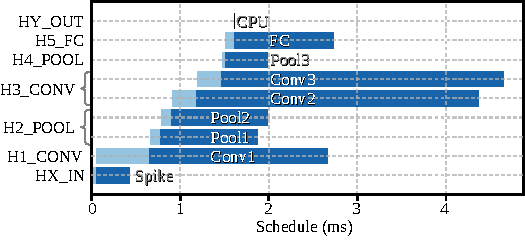
\includegraphics[width=0.75\linewidth]{../chapters/sbs_accelerator/figures/latency_pu_fp.pdf} % Adjust path and size as needed
					\caption{Performance of processing units with standard floating-point with \textbf{acceleration of 10.7X} }
				\end{figure}
				\pause
			\end{minipage}
			
			% Bottom right image
			\begin{minipage}[c][.45\textheight][c]{\linewidth}
				\centering
				\begin{figure}
					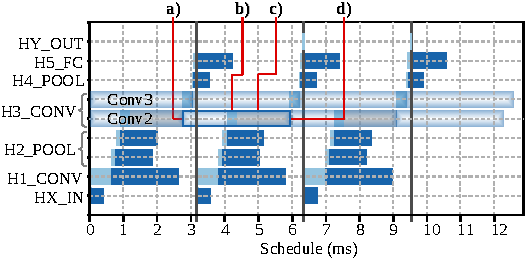
\includegraphics[width=0.75\linewidth]{../chapters/sbs_accelerator/figures/latency_fp_cycle.pdf} % Adjust path and size as needed
					\caption{Performance bottleneck of cyclic computation on processing units with standard floating-point}
				\end{figure}
			\end{minipage}
		\end{column}
	\end{columns}
\end{frame}

\begin{frame}{Deployment with Custom Floating-Point}
	\begin{columns}[c] % The [T] option aligns the tops of the columns
		
		% Left column for the first image
		\begin{column}<1->{0.5\textwidth}
			\begin{figure}
				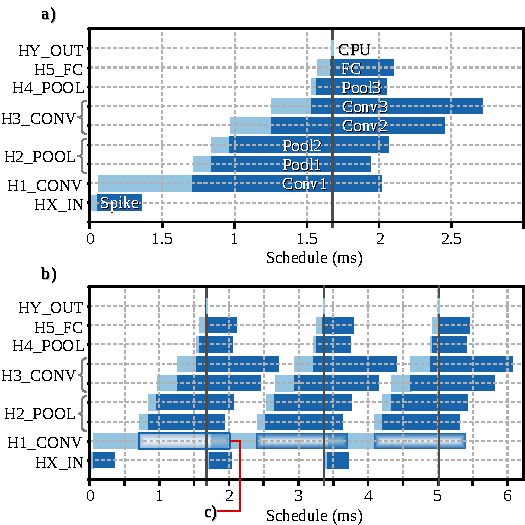
\includegraphics[width=0.75\textwidth]{../chapters/sbs_accelerator/figures/latency_cfp_cycle.pdf}
				% Adjust the filename
				\caption{Performance on processing units with hybrid \textbf{8-bit floating-point} with \textbf{acceleration of 20.5X}}
			\end{figure}
		\end{column}
		
		% Right column for the second image
		\begin{column}<2->{0.5\textwidth}
			\begin{figure}
				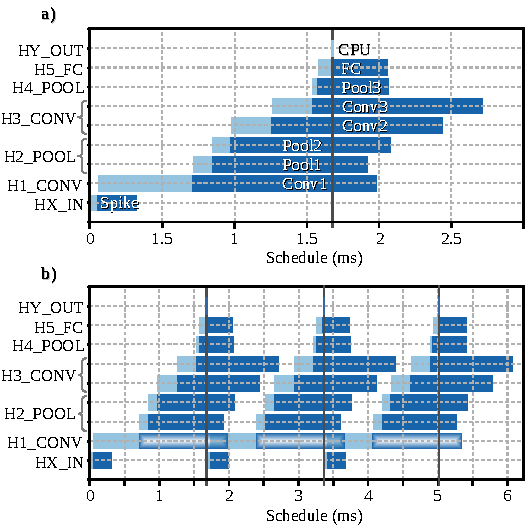
\includegraphics[width=0.75\textwidth]{../chapters/sbs_accelerator/figures/latency_log_cycle.pdf}
				\caption{Performance of processing units with hybrid \textbf{4-bit logarithmic} with \textbf{acceleration of 20.5X}}
			\end{figure}
		\end{column}
		
	\end{columns}
\end{frame}

\begin{frame}{Quantization Impact: Noise Tolerance}
	\begin{columns}
		% First column
		\begin{column}{0.33\textwidth}
			\centering
			\begin{figure}
				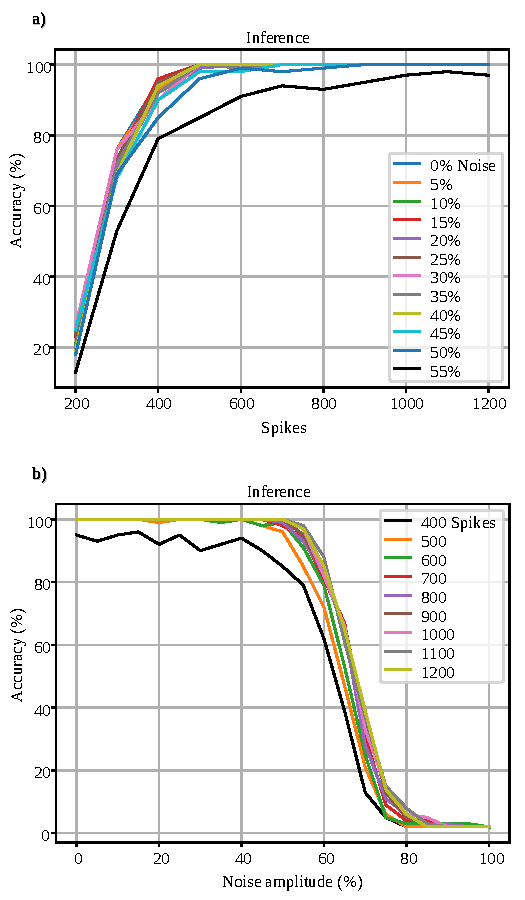
\includegraphics[width=0.75\linewidth]{../chapters/sbs_accelerator/figures/accuracy_vs_noise_pu_fp.pdf} % Adjust path and size as needed
				\caption{ Noise tolerance with \textbf{32-bit floating-point}}
			\end{figure}
			\pause
		\end{column}
		
		% Second column
		\begin{column}{0.33\textwidth}
			\centering
			\begin{figure}
				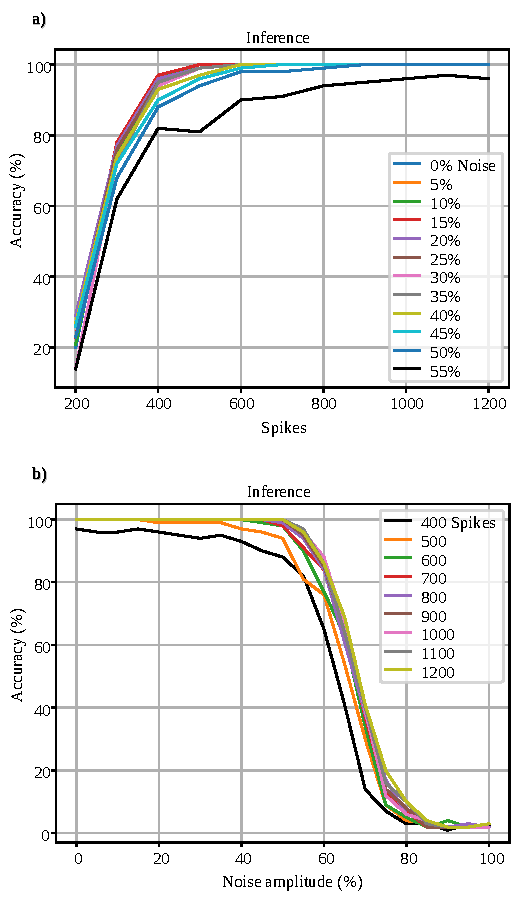
\includegraphics[width=0.75\linewidth]{../chapters/sbs_accelerator/figures/accuracy_vs_noise_pu_cfp(4-bit-exponent_1-bit-mantissa).pdf} % Adjust path and size as needed
				\caption{ Noise tolerance with hybrid \textbf{8-bit floating-point}}
			\end{figure}
			\pause
		\end{column}
		
		% Third column
		\begin{column}{0.33\textwidth}
			\centering
			\begin{figure}
				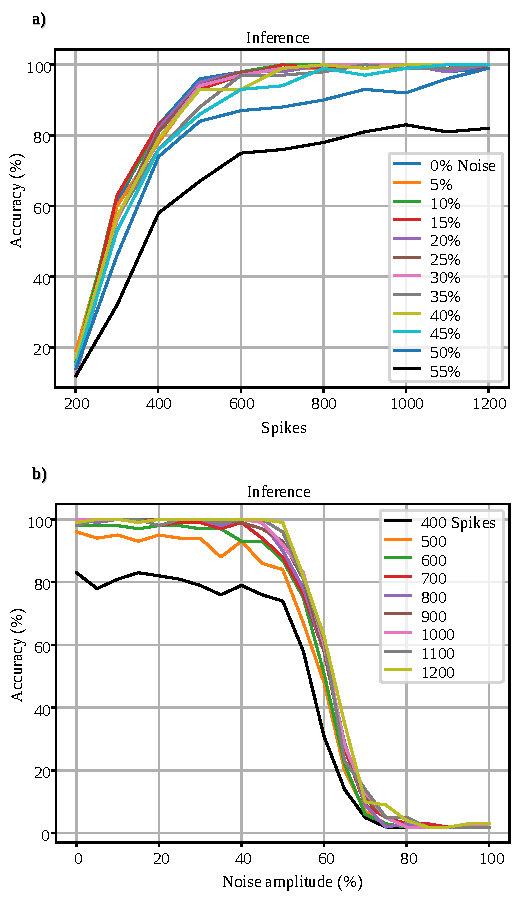
\includegraphics[width=0.75\linewidth]{../chapters/sbs_accelerator/figures/accuracy_vs_noise_pu_log.pdf} % Adjust path and size as needed
				\caption{ Noise tolerance with hybrid \textbf{4-bit logarithmic}}
			\end{figure}
		\end{column}
	\end{columns}
\end{frame}

\begin{comment}

\begin{frame}[shrink=30]{Accelerator Implementations} % Title of the slide
\begin{center} % Ensure the table is centered in the slide
\begin{threeparttable}
\caption{Accelerator implementations.} % Caption of the table
\scriptsize % Reduce the font size of the table
\begin{tabular}{lrrrrr}
\toprule
\textbf{Platform implementation} & \textbf{Power (W)} & \textbf{Clk (MHz)} & \textbf{Latency (ms)} & \textbf{Acceleration} & \textbf{Accuracy (\%)} \\
\midrule
Standard floating-point & 2.420 & 200 & 3.18 & 10.7x & 98.98 \\
Hybrid floating-point 8-bit & 2.369 & 200 & 1.67 & 20.5x & 98.97 \\
Hybrid Logarithmic 4-bit & 2.324 & 200 & 1.67 & 20.5x & 98.84 \\
\bottomrule
\end{tabular}
\end{threeparttable}
\end{center}
\end{frame}

\end{comment}


\begin{frame}{Tensor Processor On-Chip Memory}
	\begin{columns}[c] % The [T] option aligns the tops of the columns
		% Left column for equations
		\begin{column}{0.5\textwidth}
			
			\vspace{1mm}
			\begin{equation}
			TP_{M}=TP_B+V_{M}
			\end{equation}
			\vspace{1mm} 
			\begin{equation}
			TP_{B}=Input_{M}+Filter_{M}+Bias_{M}
			\end{equation}
			\vspace{1mm} 
			\begin{equation}
			Input_{M}=K_{H}W_{I}C_{I}BitSize_{I}
			\end{equation}
			\vspace{1mm} 
			\begin{equation}
			Filter_{M}=C_{I}K_{W}K_{H}C_{O}BitSize_{F}
			\end{equation}
			\vspace{1mm} 
			\begin{equation}
			Bias_{M}=C_{O}BitSize_{B}
			\end{equation}
			\vspace{1mm} 
			\begin{equation}
			C_{O}=\frac{TP_{M}-V_{M}-K_{H}W_{I}C_{I}BitSize_{I}}{C_{I}K_{W}K_{H}BitSize_{F}+BitSize_{B}}
			\end{equation}
		\end{column}
		
		% Right column for the image
		\begin{column}{0.5\textwidth}
			\begin{figure}
				\centering
				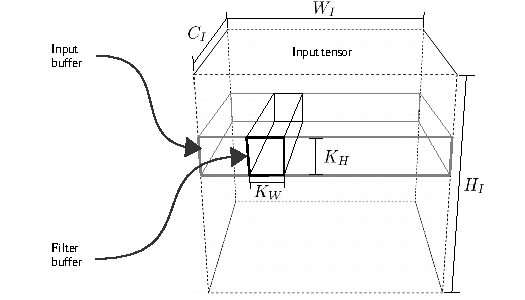
\includegraphics[width=0.9\textwidth]{../chapters/cnn_accelerator/figures/accelerator_buffers.pdf} % Adjust the filename
				\caption{ On-chip memory buffers}
			\end{figure}
		\end{column}
	\end{columns}
\end{frame}


\begin{frame}{Custom Floating-Point Quantization}
	\begin{figure}
		\centering
		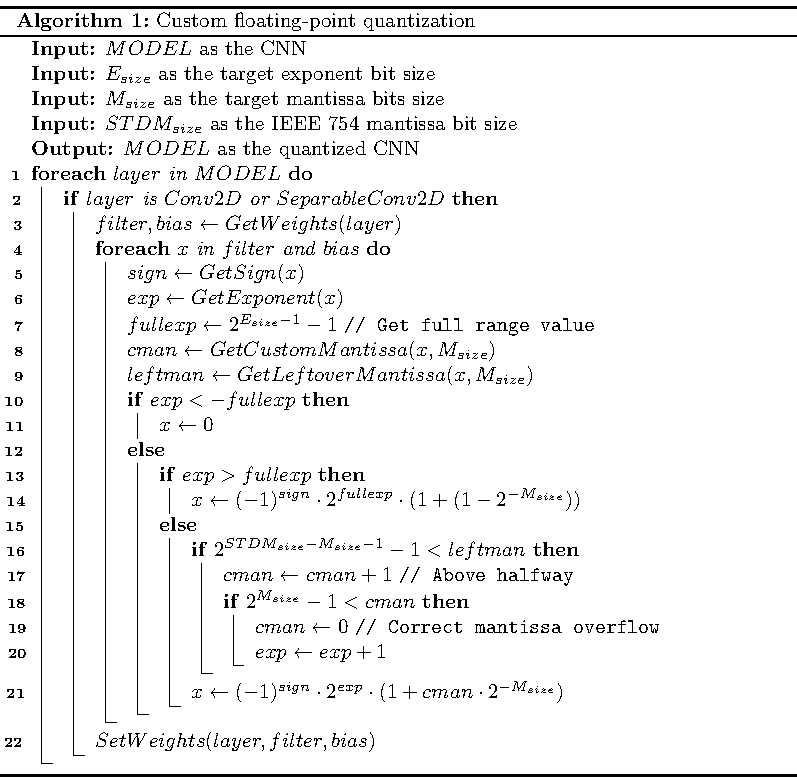
\includegraphics[width=0.6\columnwidth]{slides/algorithm_fp_2.pdf}
	\end{figure}
	
\end{frame}

\begin{frame}{Tensor Processor Setup Data Frame}
	
	\begin{figure}
		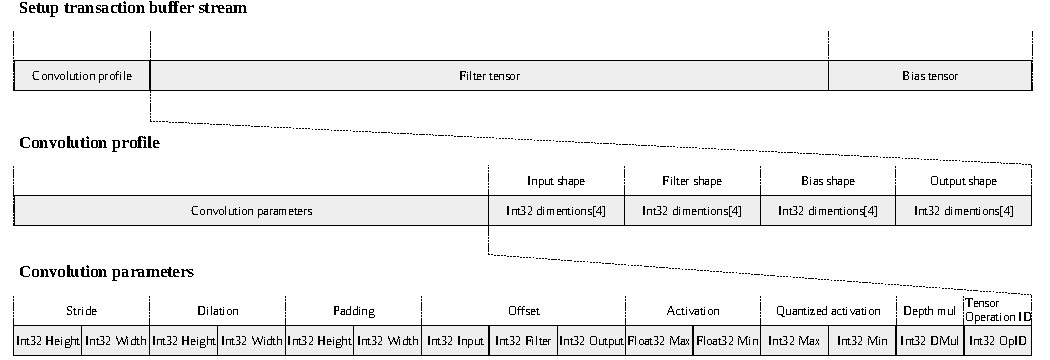
\includegraphics[width=\textwidth]{../figures/setup_transaction_buffer_stream.pdf}
		\caption{Setup transaction buffer stream}
	\end{figure}
	
\end{frame}


\begin{frame}{Embedded System Architecture with Tensor Processor}
	\begin{figure}
		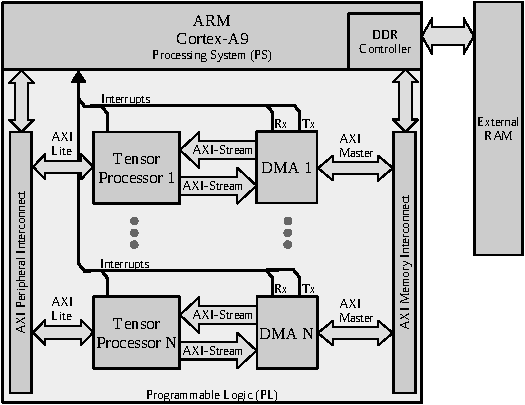
\includegraphics[width=0.75\textwidth]{../chapters/cnn_accelerator/figures/system_design.pdf} % Adjust the filename
		\caption{Embedded system architecture}
	\end{figure}
\end{frame}

\begin{frame}{Quantized Aware Training with Custom Floating-Point}
	\begin{columns}
		\column{0.5\textwidth}
		\centering
		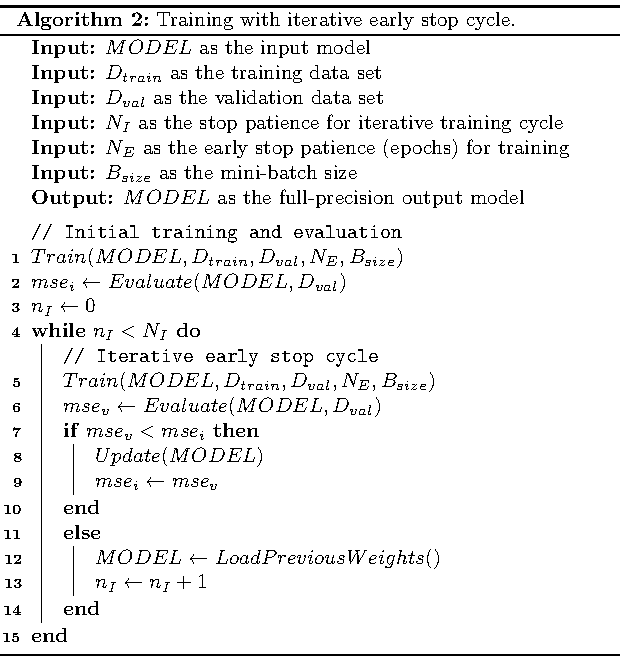
\includegraphics[width=0.65\linewidth]{slides/algorithm_early_stop_1.pdf} % Top left image
		
		\column{0.5\textwidth}
		\centering
		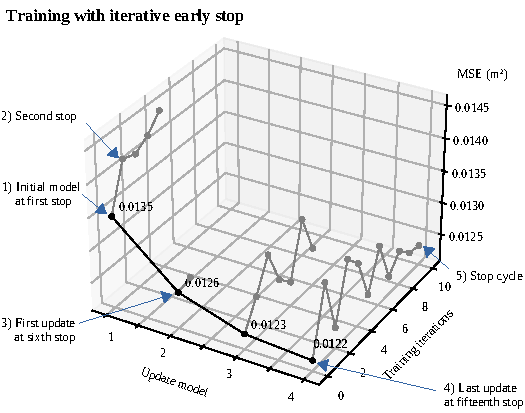
\includegraphics[width=0.65\linewidth]{slides/figures/training_iterative_early_stop.pdf} % Top right image
	\end{columns}
	\pause % Pause after top images to reveal bottom images together
	\begin{columns}
		\column{0.5\textwidth}
		\centering
		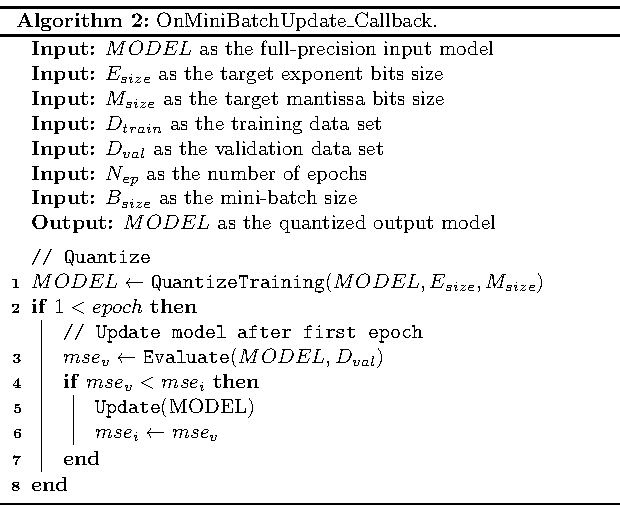
\includegraphics[width=0.65\linewidth]{slides/OnMiniBatchUpdate_2.pdf} % Bottom left image
		
		\column{0.5\textwidth}
		\centering
		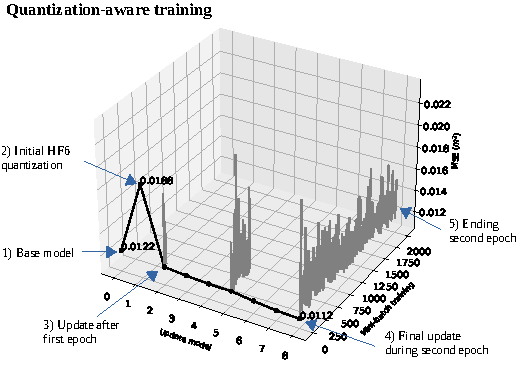
\includegraphics[width=0.65\linewidth]{slides/figures/QAT.pdf} % Bottom right image
	\end{columns}
\end{frame}

\begin{frame}
	\frametitle{Comparison with Related Work with Tensor Processor} % optional, remove or leave empty if no title is desired
	\begin{center}
		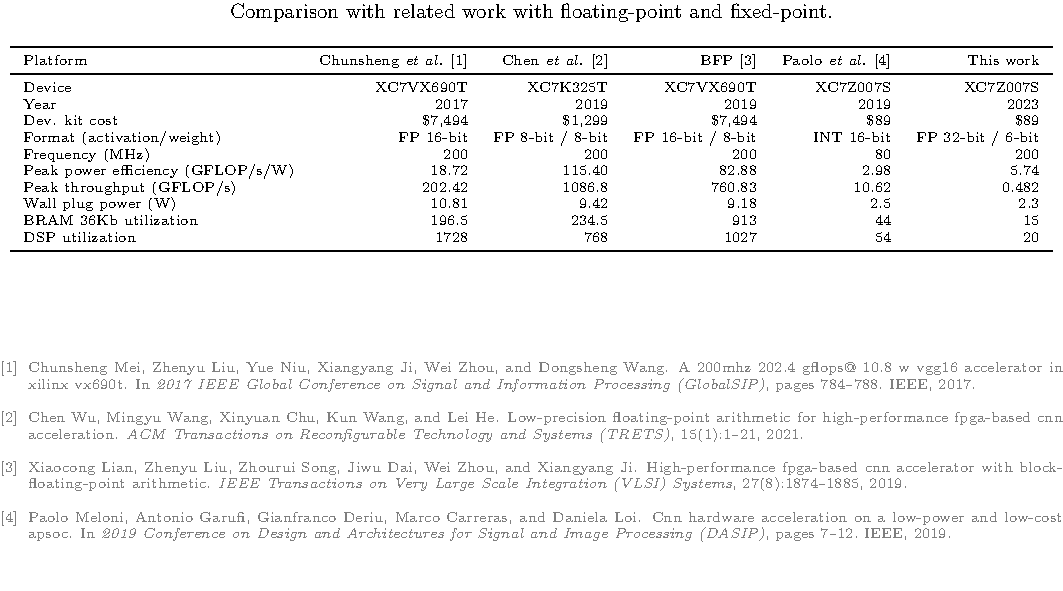
\includegraphics[width=\textwidth]{slides/figures/cnn_related_work.pdf} % Adjust the width as needed
	\end{center}
\end{frame}

\backupend